\chapter{Open Microfluidics for Education}
\label{App:OpenMicrofluidics}

\section{Introduction}

\subsection{Big trouble in little channels}
Microfluidics can be a scary word for many people. Mention microfluidics to someone who has never heard the term before and there will be nothing but blank faces. Discuss it with those slightly familiar with the field and responses can include responses like, "magic", "that sounds hard", and "uh huh". The word, microfluidics to those doing microfluidics research will conjure images of rows of pumps, tangled webs of tubing, and the dreaded experiment-destroying bubbles.

In 2009, Holger Becker lamented that microfluidics was just to immature of a technology to have a "killer app" and break into the mainstream and predicted that it would be at that point sometime between 2014 and 2019 \cite{Becker2009HypeMicrofluidics}. In 2014, Theranos Inc. achieved a \$9 billion valuation with the promise that it would revolutionize the blood testing industry, being able to perform dozens of assays from a single finger prick, and it was all achieved through microfluidics. It appeared as Becker's prediction was correct and microfluidics was finally beginning to enter the popular lexicon. The public's positive association with microfluidics was short lived as Theranos was unable to deliver accurate results on any of the assays it was developing. The company lost its massive valuation, has been sued, sanctioned by the FDA, and is now subject of a film starring Jennifer Lawrence as the company's founder, Elizabeth Holmes \cite{Stockton2016}. The lack of public understanding of what microfluidics is combined with the negative media coverage can lead one to the conclusion that the field of microfluidics has considerable public relations issues. While being unpopular is not inherently bad for microfluidics, a negative public opinion on the field is. Negative public opinion could lead potential researchers away from microfluidics research and possibly endanger the future of funding in the field. In the current climate the next "killer app" enabled by microfluidics will need to have its inner-workings deeply hidden from view and would do well to avoid using "microfluidics". Microfluidics needs to change its perception to continue to grow and advance.

\subsection{Teaching with microfluidics}
An approach to get people to understand microfluidics principles and get them excited about the subject is the use of classroom educational tools. These tools can be as mundane as the a classroom lecture, involve student-level device fabrication like gelatin (Jell-O) microchannels \cite{Yang2013}, or can give students the full microfluidic blackbox experience with complete pump-driven systems capable of doing droplet microfluidics from companies like Dolomite. Modular systems like breadboard microfluidics have also been introduced to educational settings, however, they also have high entry costs and require extensive setup and preparation time \cite{Chen2011, Shaikh2005, Chen2014, Langelier2011, Papautsky2008}. Each technique has advantages, unfortunately the techniques that result in the highest level of student engagement involve the most effort from the instructor to prepare or are prohibitively expensive for many programs \cite{Fintschenko2011Education:Laboratory}. 

We present a modular microfluidic platform that aims to teach students many microfluidics principles in a hands-on learning environment that maximizes student engagement while reducing instructor effort and institutional cost. The platform utilizes the high surface tension of water at the air-liquid interface and capillary action to drive fluid flow through across open microchannels. The microchannels are engineered onto the surface of modular interconnectable blocks to create microfluidic circuits as described in Chapter \ref{Chap:OpenMicrofluidics}.

\section{Methods}

\subsection{Device design and fabrication}
The microfluidic channel design and block interface are discussed in Chapter \ref{Chap:OpenMicrofluidics}. The blocks themselves are designed to interface and exchange fluids without bonding or any permanent connections so they can reconfigured during operation, reorganized by the user to achieve different functions, and reused for future learning experiences. The choice of a Lego-based interface for the  blocks was designed to be simple to use, and familiar so little training on the part of the instructor and student were needed to learn how to interact with the blocks and create microfluidic circuits. Each of the blocks were designed to perform a microfluidic function. The functions included in the study are dispensing, mixing, valving, combining, and splitting. These basic functions can be used to create an array of different microfluidic circuits capable of achieving different goals. 
Also included in this study was the cross section channel device discussed in Chapter \ref{Chap:OpenMicrofluidics}. This device was used to introduce students to the concept of capillary flow in open microchannels with different surfaces and to help them understand the conditions for capillary flow described in the Generalized Cassie Law \cite{Casavant2013, Berthier2015a} and prepare them to create more complicated constructs with the microfluidic blocks.

All parts used in the study were 3D printed with Accura 25 (a resin with polypropylene-like properties) using stereolithography and sourced from Midwest Prototyping (Bluemounds, WI). Prior to instruction, devices were plasma treated with oxygen plasma to increase their hydrophilicity and allow better flow in the devices.

\subsection{Study design}
The students used in this study were in a college-level course on microfluidics and had prior knowledge of many microfluidics concepts before the session, in response the session included minimal explanation of more general concepts. The course was designed as a 45 minute session. The first 5 minutes were used to mathematically explain the conditions for spontaneous capillary flow in microchannels. The next 10 minutes were used for the students to explore spontaneous capillary flow using the cross section capillary flow channels. In the next 20 minutes of the session, students were divided into groups of 3 and 4 and given a set of microfluidic blocks that included one of each of the functional blocks described above. The final 15 minutes were spent with students demonstrating their circuits to the instructor and each other, discussing what worked, what didn't, and their thoughts on why. The instructor had minimal intervention into the student assignments making themself available when students requested assistance. 

Following the instruction session, students filled out a survey evaluating their experience with the microfluidic blocks designed to measure several components of their experience with the educational session. The survey questions were obtained from surveys developed to evaluate the effectiveness of new teaching tools. The specific questions were designed to determine the educational value of the blocks, student engagement with the blocks, target audience for the blocks, and whether the blocks were appropriate for a classroom setting. Surveys were completed and returned by 17 of the 20 students who participated in the educational session. Data from the surveys was collected and aggregated to preserve student anonymity.

\section{Results and discussion}

\subsection{Survey results}
The main metric for evaluating the success of the platform as an engaging educational tool is the student feedback collected through the survey questions. These questions used established coding methods to ensure that student responses could be mapped back to answer questions that we cared about evaluating. The answers to the questions were in a multiple choice format where students selected the degree to which they agreed with the statement posed. The number of choices to respond to each survey question was limited to 4 or 5 instead of 10 to reduce importance biasing since this study was small (17 participants) although the authors acknowledge that this method slightly increases the Likert value \cite{ISI:000252619600006, ARMSTRONG1987, matell1971there}.

The first set of survey questions was designed to evaluate how the students interacted with the block microfluidics. These questions were focused on whether the activity was enjoyable, encouraged collaboration, and was educational (Fig. \ref{figure:EduFig1}. The results were fairly positive across all questions. Students responded that they enjoyed the activity, engaged with with students, found that the activity enabled them to pursue their own ideas, and came away learning something new about microfluidics. Students still responded positively, though not as much to the survey question that asked if they were able to relate the activity to other experiences they've had. The lowest Likert value came from the question if the students explained the activity to each other. This may seem to be in conflict with the question evaluating whether the student asked questions or talked with another student to which the response was highly positive which was meant to evaluate collaboration of the students in response to the activity. This question should have been separated into two separate questions or reduced in scope to allow for better analysis, though it still can be interpreted that this activity resulted in collaboration and discussion among the students. 

\begin{figure}[h!] %DONE
\centering
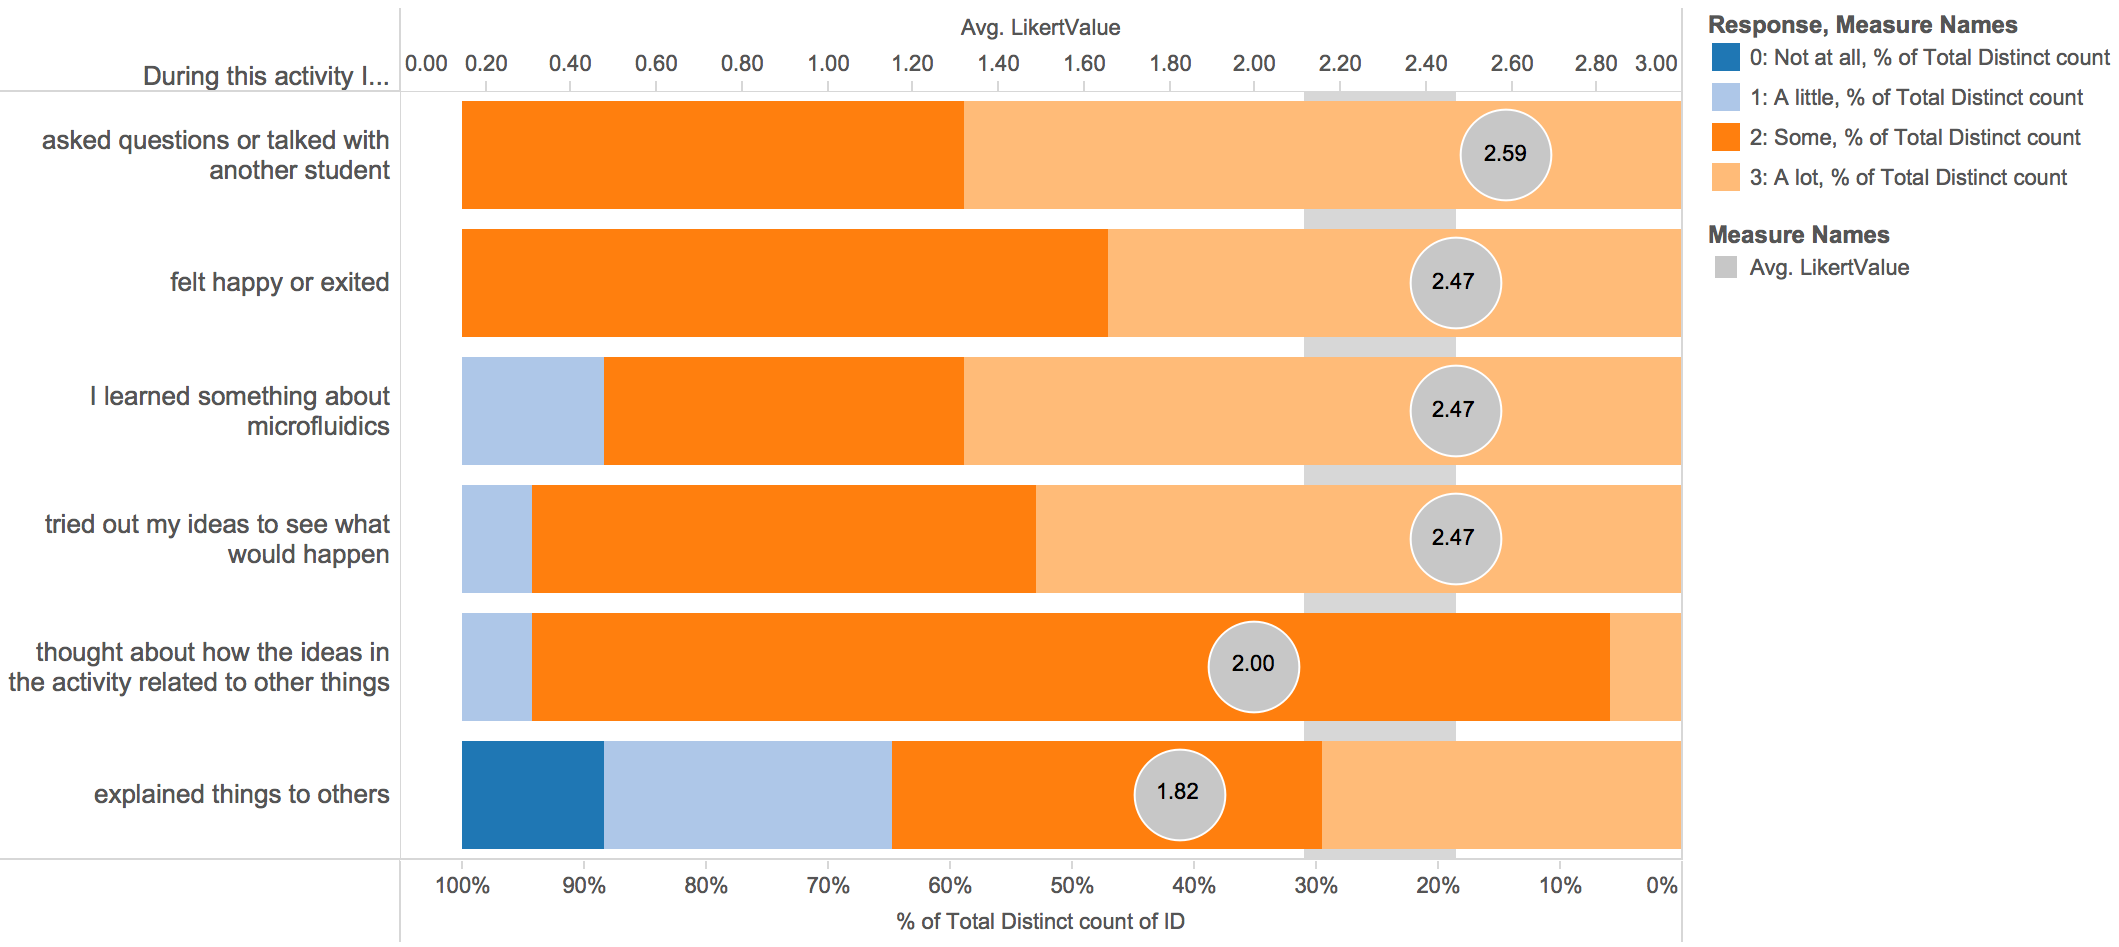
\includegraphics[width=5.9in]{/EduFig1.png}
\caption[\textbf{Responses to section of survey that evaluated student engagement, collaboration, and learning.}]{\textbf{Responses to section of survey that evaluated student engagement, collaboration, and learning.} Survey questions were all phrased with "during this activity I" and followed with responses listed in each row. The legend on the right of the figure describes the response students gave to the question. The average Likert value of each question is displayed in a gray circle. The vertical gray bar running through each row is the standard deviation from the mean for the responses to all questions displayed.}
\label{figure:EduFig1}
\end{figure}
\FloatBarrier

The second section of the survey was designed to evaluate whether the activity was appropriate for the students that were involved in it \ref{figure:EduFig2}. The students were asked whether their participation was voluntary to which all but one responded that they wanted to be involved as opposed to being forced into the activity. The second and third questions probe more directly whether the students had an appropriate level of knowledge and skill coming into the activity to make it beneficial for them. The second question, which asked how much the students knew about the subject indicated that they have all some experience in the subject area, which is to be expected as all students were concurrently enrolled in a college-level microfluidics course. The final question directly asked the students if they thought the activity was at the appropriate skill level for them. Approximately 80\% of students said that it was appropriate for their skill and knowledge level, while the rest responded that it was too easy for them. No students responded that the activity was too difficult for them. These three questions indicate that the activity may have been too easy to accomplish for students in a microfluidics class but the high percentage of students that responded they were doing the activity because they wanted to was high, indicating they still found the activity enjoyable. 

\begin{figure}[h!] %DONE
\centering
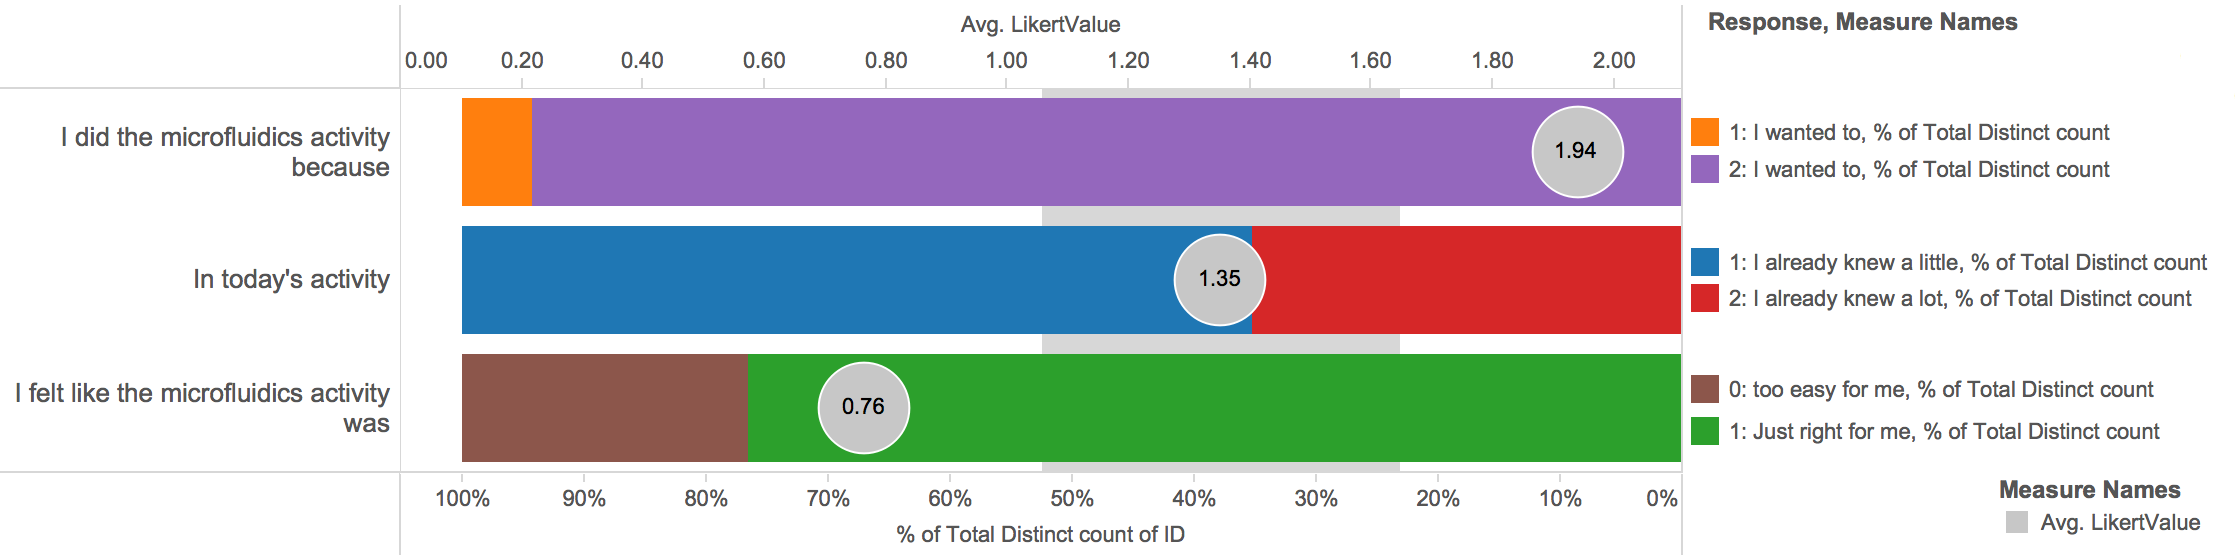
\includegraphics[width=5.9in]{/EduFig2.png}
\caption[\textbf{Response to section of survey to measure appropriateness of microfluidic blocks activity for the students participating in the activity}]{\textbf{Response to section of survey to measure appropriateness of microfluidic blocks activity for the students participating in the activity} Each row represents the responses to a question posed in the survey. The options given to respond to each question are unique and are indicated by color in the chart and to the legend to the right of each bar. The mean Likert value for each question is displayed in grey and placed at the mean of the responses for each question.}
\label{figure:EduFig2}
\end{figure}


The third set of questions asked the students who participated in the activity whether they thought that the open microfluidic blocks were well suited as an educational tool/toy and if they thought it would make a good research prototyping tool (Fig \ref{figure:EduFig3}). The feed back for all questions in this segment were highly positive. The first question, which asked if they thought the platform would make for a good prototyping tool in lab demonstrates that the do see practical applications for the platform beyond what they experienced in the activity they were participating in. The second question asked if the students thought that open microfluidic blocks were useful as a teaching tool, giving additional feedback on what they thought about the activity they had just participated in. The third question asked how they felt about open microfluidic blocks as a learning tool/toy that could be used and experienced at home. The positive response given here suggests that they found the blocks easy enough to use that direct supervision from an instructor while using the platform is unnecessary would be comfortable creating microfluidic circuits at home.

\begin{figure}[h!] %DONE
\centering
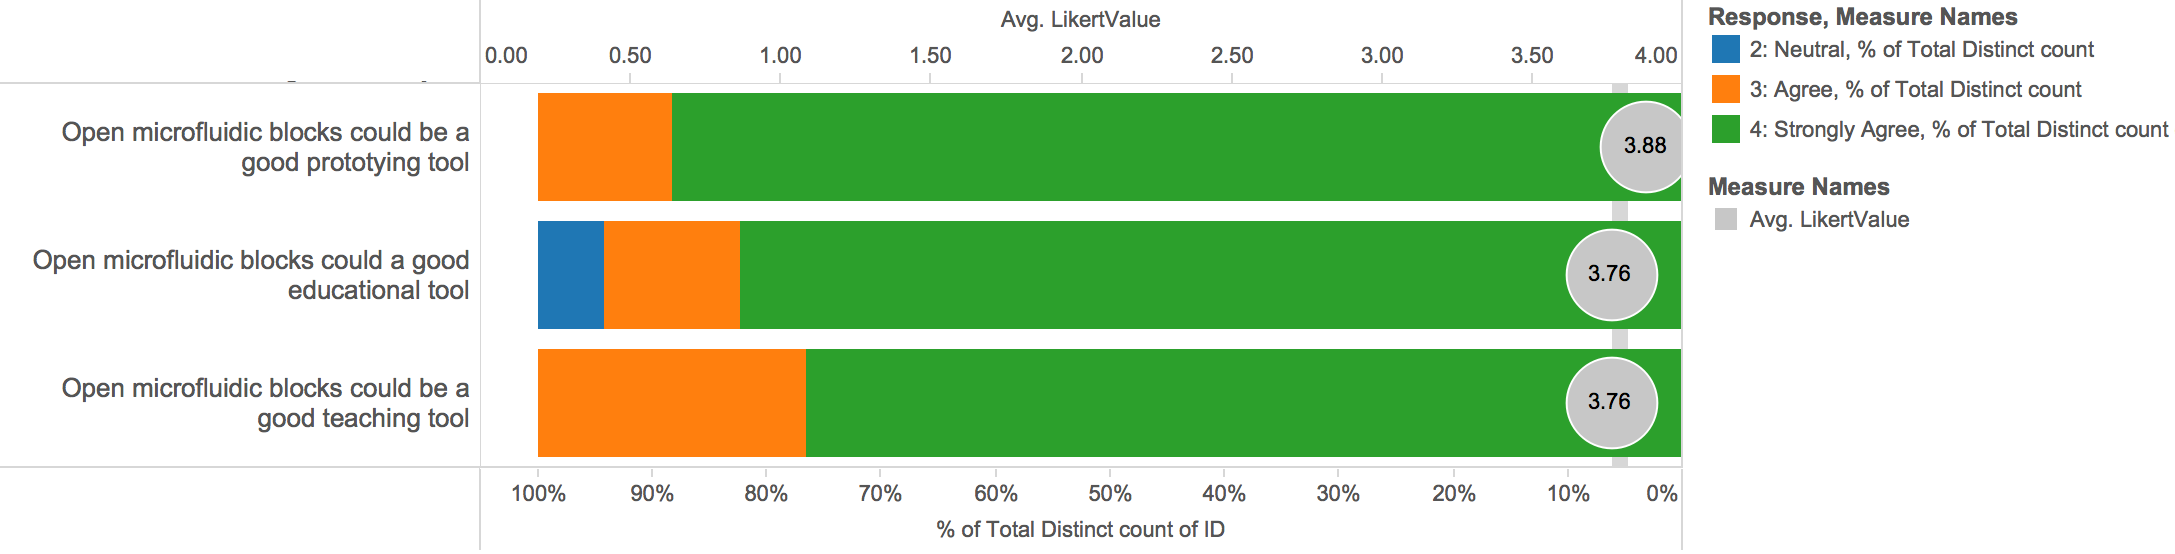
\includegraphics[width=5.9in]{/EduFig3.png}
\caption[\textbf{Response to section of survey how students felt about the practical value of the open microfluidic blocks platform}]{\textbf{Response to section of survey how students felt about the practical value of the open microfluidic blocks platform} The questions asked in this section of the survey were Do you think that... "open Microfluidic blocks could be a good teaching tool in the classroom?", "open microfluidic blocks could be a good prototyping tool for research?", and "open microfludic blocks could be a good educational toy in a home or informal learning space?". Responses were measured from 0 as "strongly disagree" to 4 as "strongly agree". The mean Likert Values for each questions is in grey and overlayed on mean response to each question asked. The mean Likert value for all questions in this section is a vertical grey bar that goes through all rows.}
\label{figure:EduFig3}
\end{figure}

\section{Conclusions and future work}
The responses to the survey were consistently positive and show that the platform has great potential as a learning to to engage and teach microfluidics in the classroom and beyond. The sample sized used in this study was relatively small and focused on a very small subset of individuals, those currently enrolled in a college-level microfluidics class. To address this limited sample size we are currently working with the Discovery Outreach program to test the platform and activity on students elementary to high school. The activity will need to be tailored to fit the group experiencing it, but it will integrate well with the established microfluidics activities that Discovery Outreach is already hosting. We hope that by reaching a larger sample size we will be able to discover flaws in the platform and make improvements to it to not only make it more robust but to improve learning outcomes from students working with the microfluidic blocks. We also did not survey for the effectiveness of the cross sectional open microfluidics device along with the brief explanation of the Generalized Cassie Law. Future studies will include those components to determine how useful they are to students if they are usefull at all.

A goal of this study was to create a tool that allowed good student engagement, good learning outcomes, but with minimal preparation to the instructor, and at minimal cost. The open microfluidic blocks used in this study were 3D printed and delivered to us from a service. 3D printing technology makes this platform highly accessible for individuals and institutions around the country and world. The resin used in printing these parts, Accura 25, is fairly hydrophobic, however, there are more hydrophilic resins available for printing which eliminate the need for plasma treatment (a technique with a relatively high cost of investment) of the blocks before use. The blocks were also designed to be compatible with injection molding techniques so that mass production of the platform is feasible which would considerably lower the cost-of-entry for access to the blocks. 

Our ultimate goal with the open microfluidic blocks platform is to create a tool that not only engages people, and helps them learn, but to make microfluidics fun, to make it a subject that individuals want to learn more about. If these results we achieved in this pilot study continue to receive the same feedback as the sample size and scope is expanded we will be well on our way from turning microfluidics from a dirty word into something people are excited about.

\section{Acknowledgements}
We would like to thank Dr. Yan Wu for organizing the microfluidics learning event, without that, this endeavor would have never been possible, Jay Ludden for introducing the idea of educational outreach as an use for the open microfluidic blocks, as well as vetting the survey questions and assembling the lesson plan, and Travis Tangen of Discovery Outreach for his valuable expertise and input in educational outreach.

\begin{figure}[h!] %DONE
\centering
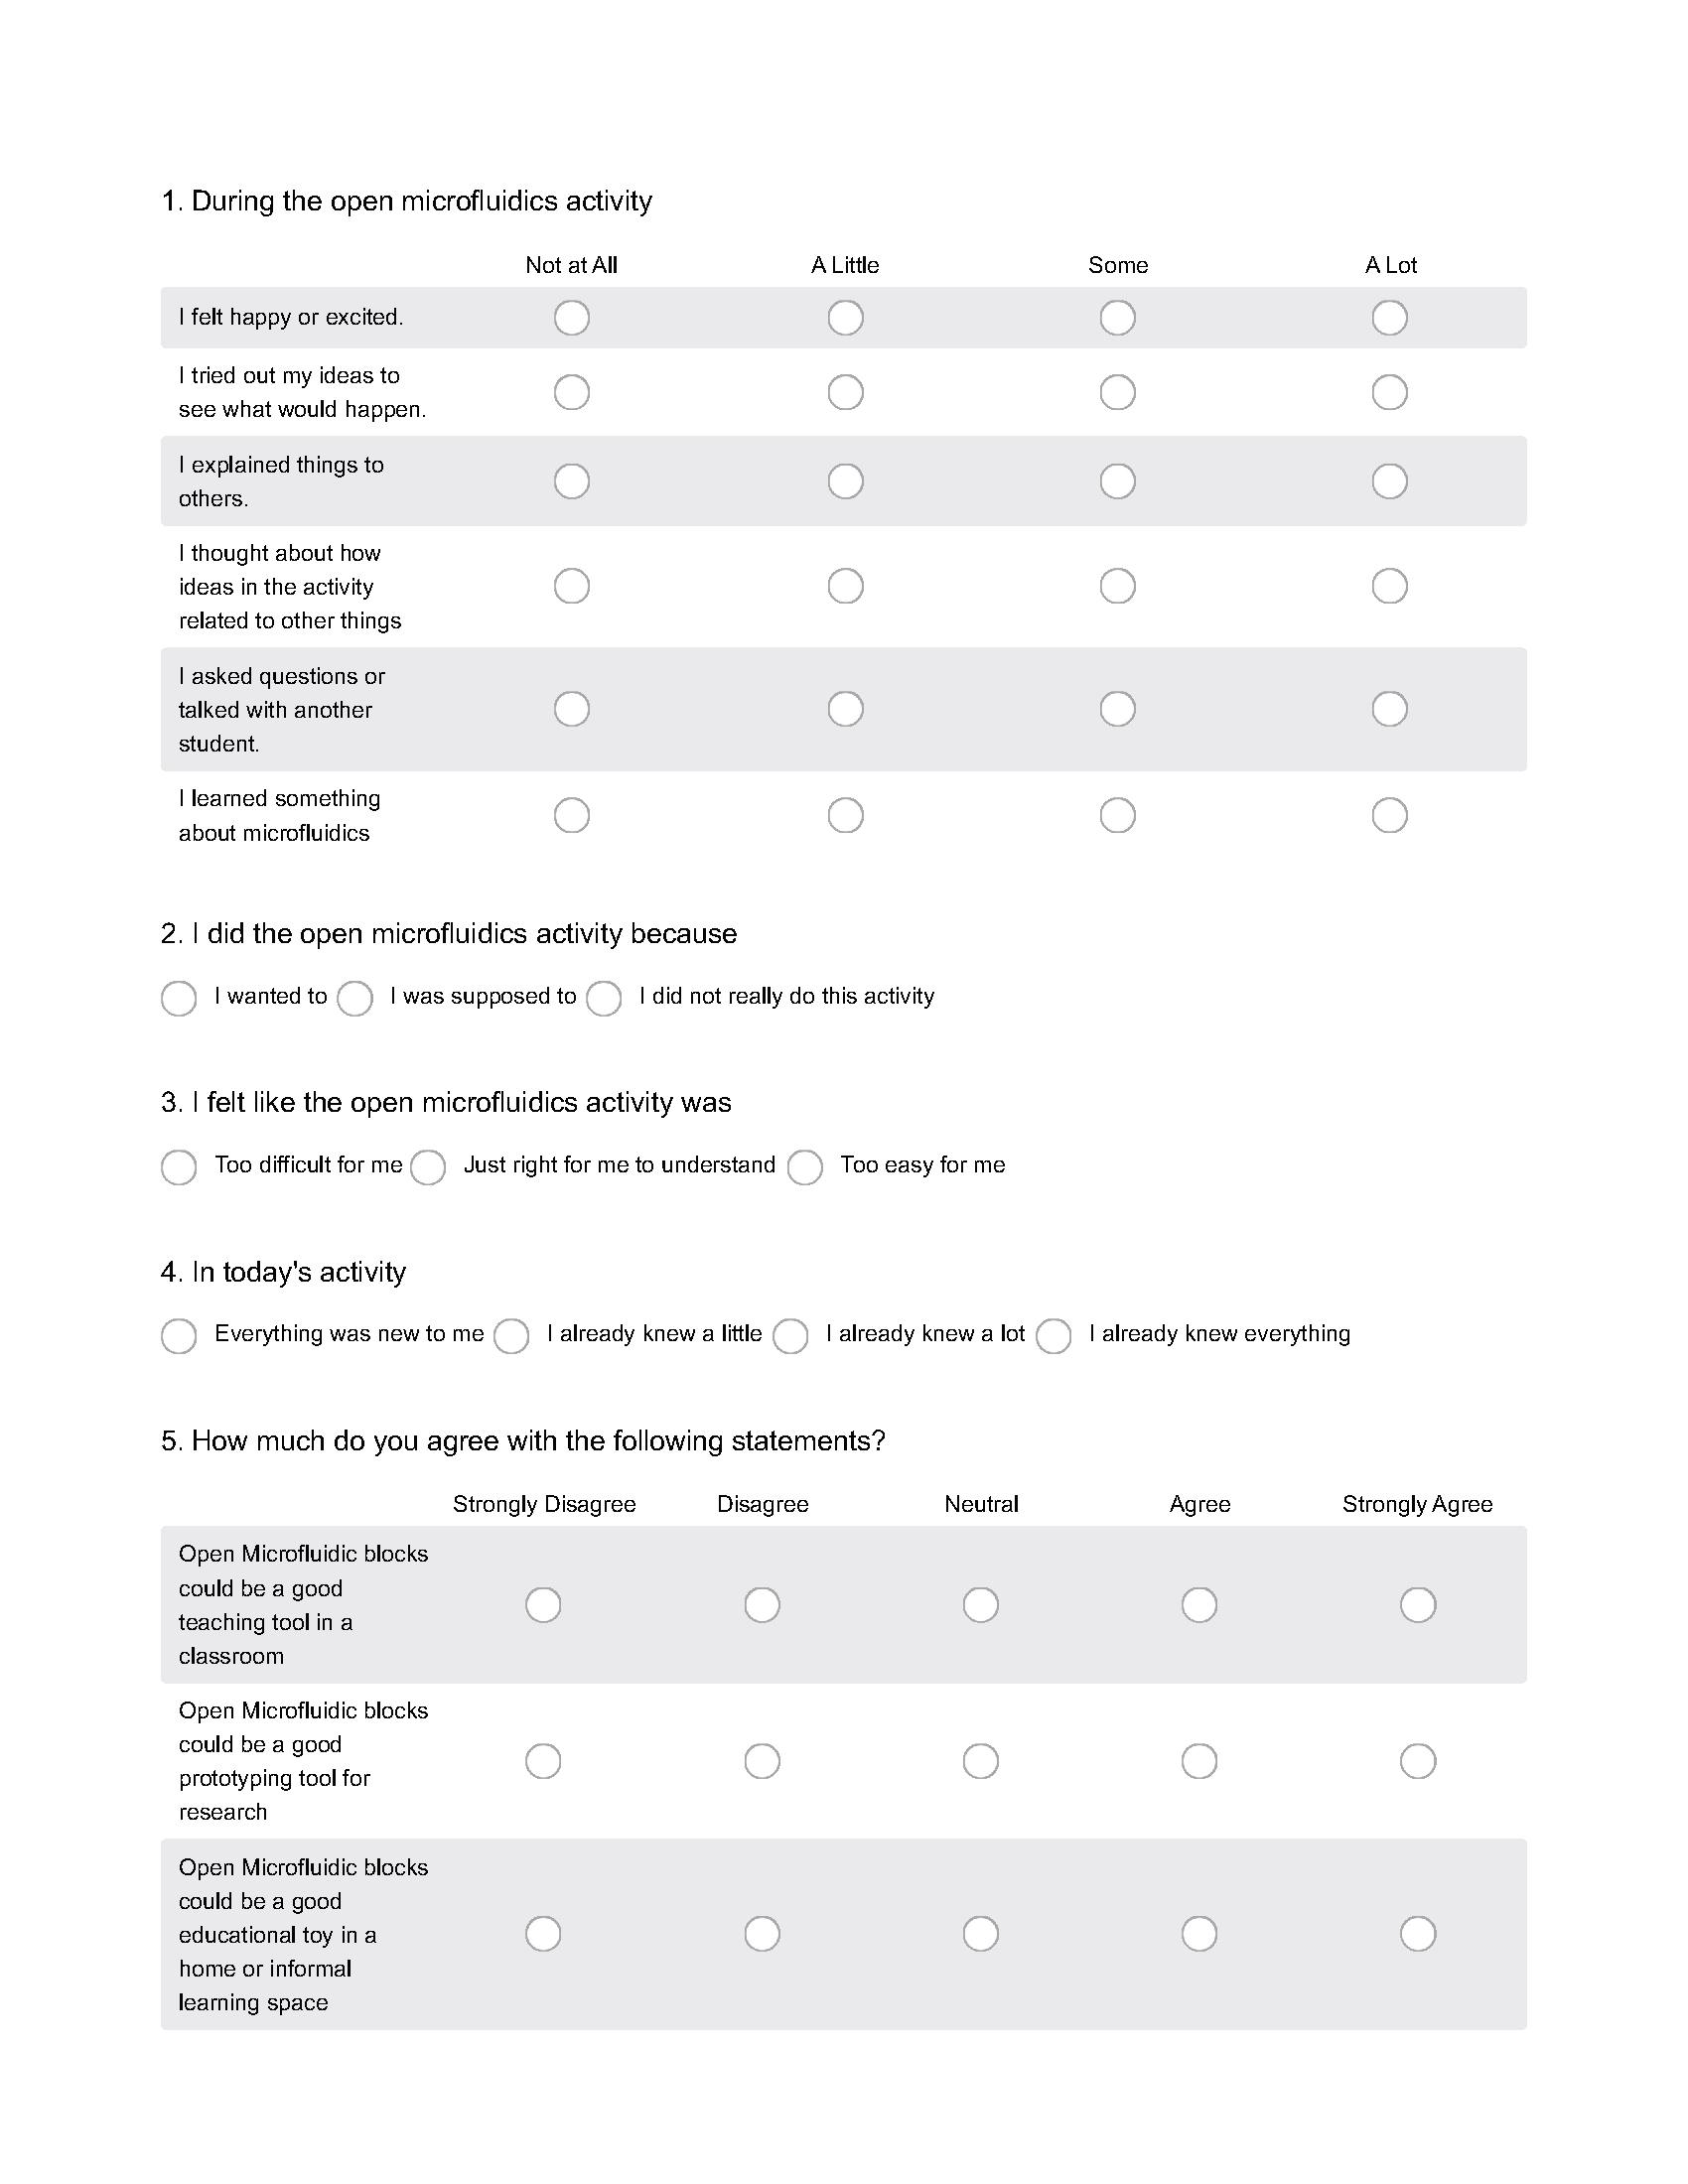
\includegraphics[width=6in]{/survey.png}
\caption[\textbf{Survey for open microfluidic blocks activity}]{\textbf{Survey for open microfluidic blocks activity}}
\label{figure:survey}
\end{figure}






